\documentclass[11pt,a4paper,titlepage]{article}
\usepackage[utf8]{inputenc}
\usepackage[dutch]{babel}
\usepackage{amsmath}
\usepackage{amsfonts}
\usepackage{amssymb}
\usepackage{graphicx}
\usepackage{hyperref}
\usepackage{algorithm}
\usepackage{algpseudocode}\usepackage{float}
\usepackage{fullpage}
\renewcommand{\familydefault}{\sfdefault}

\algblockdefx{ForEach}{EndForEach}[2]{\textbf{for each} #1 \textbf{in} #2 \textbf{do}}{\textbf{end for}}

\author{Pieter-Jan Coenen en Stijn Caerts}
\title{Practicum Toepassingen van Meetkunde in de Informatica \\ Snijdende rechthoeken}
\date{20 mei 2016}

\begin{document}
	\maketitle
	\tableofcontents
	\newpage
	\section{Beschrijving algoritmen}
	\subsection{Algoritme 1}
	\emph{Algoritme 1} is een brute-force algoritme. Elke rechthoek wordt gecontroleerd met elke andere rechthoek voor snijding. Om te vermijden dat we twee rechthoeken dubbel controleren op snijpunten, houden we een lijst bij van de rechthoeken waarvoor we snijpunten met alle andere rechthoeken al zijn nagegaan. In pseudocode ziet dat er uit als volgt.
	\begin{algorithm}[H]
		\caption{}
		\begin{algorithmic}[1]
			\State intersections $\gets \varnothing $
			\State checked $\gets \varnothing $
			\ForEach {rect1} {rectangles}
				\ForEach {rect2} {rectangles}
					\If {rect1 $\neq$ rect2 \textit{and} rect2 $\notin$ checked}
						\State intersections $ \gets $ intersections $ \cup $ calculateIntersections(rect1, rect2)
					\EndIf
				\EndForEach
				\State checked $\gets$ checked $\cup$ rect1
			\EndForEach
		\end{algorithmic}
	\end{algorithm}
	Aangezien we twee geneste lussen hebben, en we niet dubbel controleren voor eenzelfde paar rechthoeken. De functie \emph{calculateIntersections()} wordt daarom $ (n-1) + (n-2) + \dots + 2 + 1 = \frac{n(n-1)}{2} $ keer uitgevoerd en dus heeft \emph{Algoritme 1} een complexiteit van $\mathcal{O}(n^2)$.
	
	\subsection{Algoritme 2}
	\begin{algorithm}[H]
		\caption{}
		\begin{algorithmic}[1]
			\State intersections $\gets \varnothing $
			\State queue $\gets$ lijst van rechthoeken gesorteerd op x-coördinaat.
		\end{algorithmic}
	\end{algorithm}
	\section{Experimenten en correctheid}
		\subsection{Experimenten}
		We hebben verschillende experimenten uitgevoerd om de complexiteit en werking van onze algoritme na te gaan. Eerste hebben we een doubeling experiment uitgevoerd waarbij de x- en y-coördinaten van de hoekpunten tussen 0 en 1 liggen.  Nadien hebben opnieuw verschillende doubeling experimenten uitgevoerd waarbij eerst de x- en y-coördinaten van de hoekpunten tussen 0 en 0,2 liggen, daarna tussen 0 en 0.5 en vervolgens laten we de waardes van de hoekpunten variëren tussen 0 en 0.75.
			\subsubsection{Doubeling experiment met hoekpunten tussen 0 en 1}
				We hebben een doubeling experiment uitgevoerd waarbij het aantal rechthoeken laten toenemen vanaf 1 tot 8192.  We hebben hierbij de tijd in miliseconden gemeten die de drie algoritme nodig hebben om de snijpunten van de rechthoeken te vinden.
				\begin{figure}[H]
				\centering
				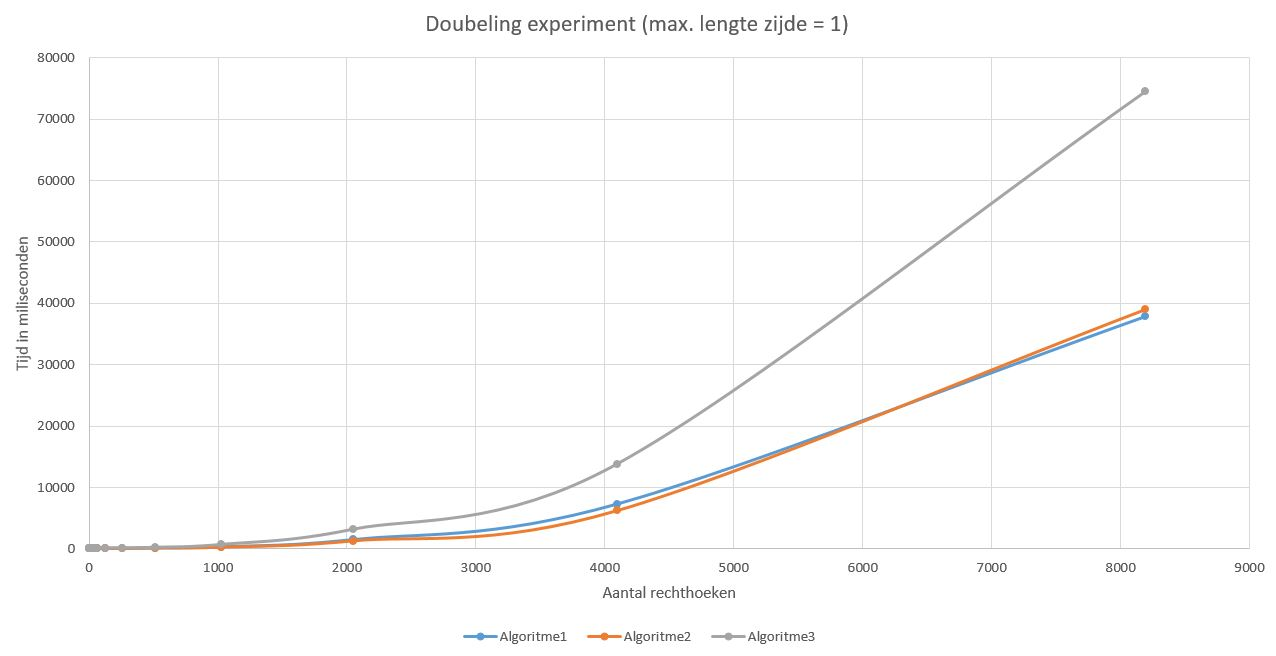
\includegraphics[width=0.75\textwidth]{zijde1.JPG}
				\caption{\label{fig:convR}Grafiek voor het doubeling experiment met zijde die variëren tussen 0 en 1}
				\end{figure}
			\subsubsection{Doubeling experiment voor verschillende lengtes van de zijden}
				OOk hier hebben we een doubeling experiment uitgevoerd.  We hebben hierbij de tijd in miliseconden gemeten die de drie algoritme nodig hebben om de snijpunten van de rechthoeken te vinden. We hebben dit experiment eerst gedaan voor zijdes met een maximale lengte van 0.01, dan voor zijdes met een maximale lengte van 0.1, vervolgens voor zijdes met een maximale lengte van 0.2 en tot slot voor zijdes met een maximale lengte van 0.5.\\ \\
				We verkregen de volgende grafieken:
				\begin{figure}[H]
				\centering
				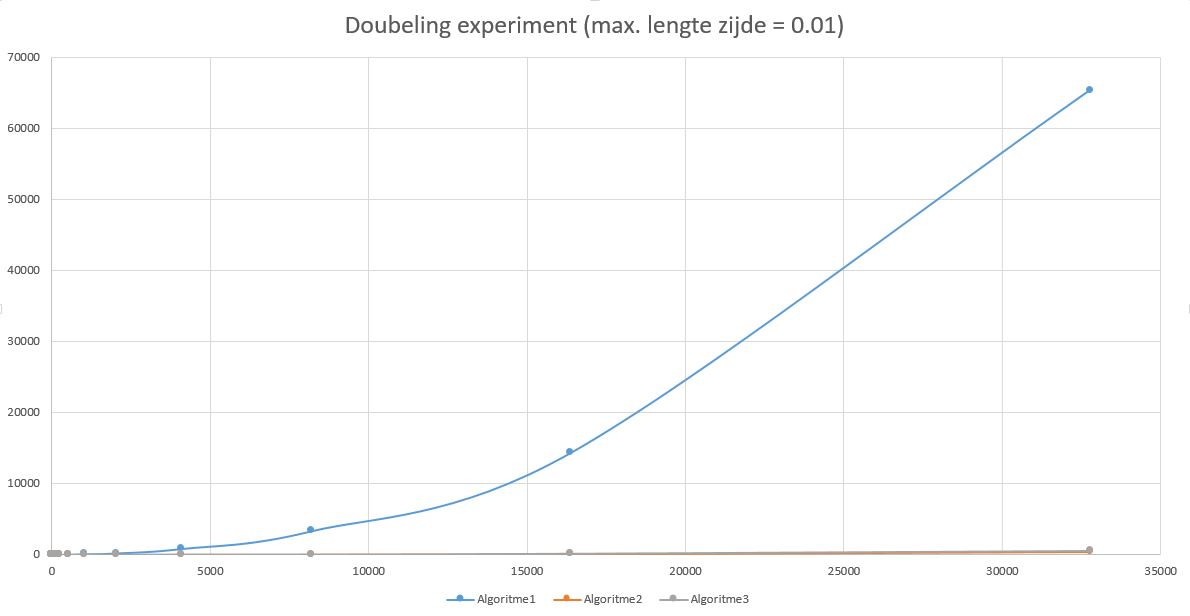
\includegraphics[width=0.75\textwidth]{zijde001.JPG}
				\caption{\label{fig:convR}Grafiek voor het doubeling experiment met zijdes die variëren tussen 0 en 0.01}
				\end{figure}
				\begin{figure}[H]
				\centering
				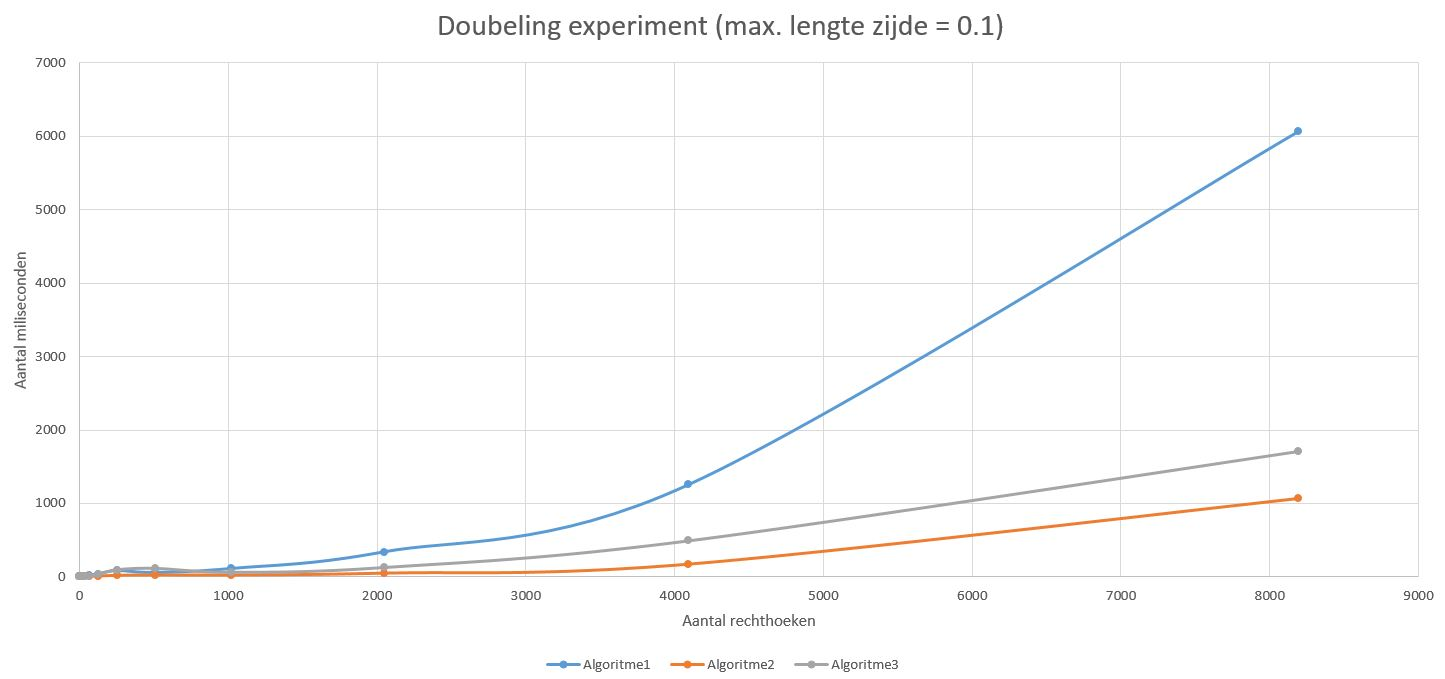
\includegraphics[width=0.75\textwidth]{zijde01.JPG}
				\caption{\label{fig:convR}Grafiek voor het doubeling experiment met zijdes die variëren tussen 0 en 0.1}
				\end{figure}
				\begin{figure}[H]
				\centering
				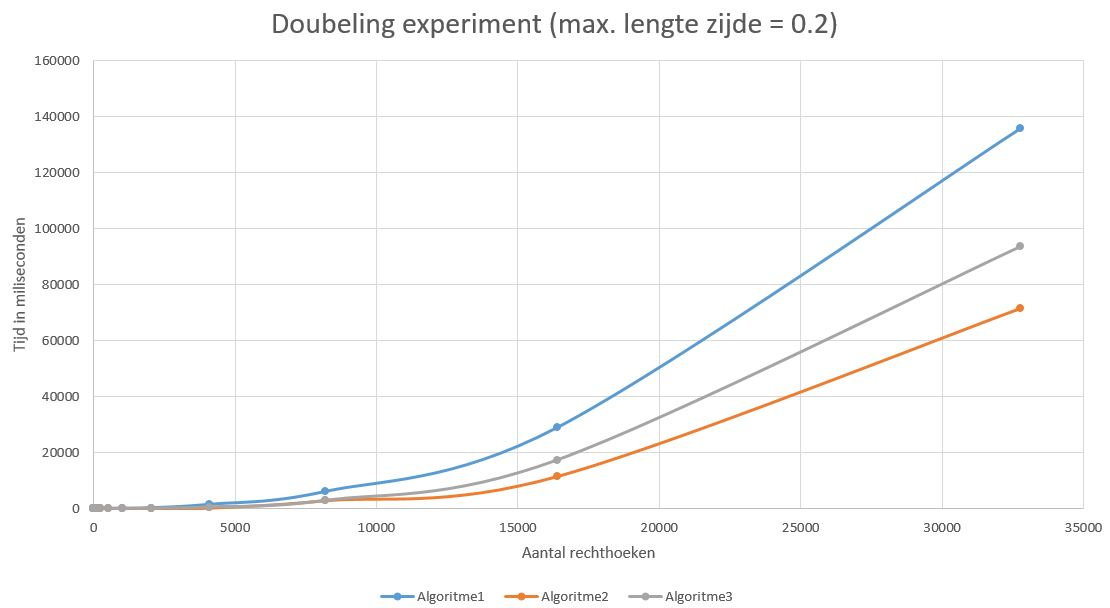
\includegraphics[width=0.75\textwidth]{zijde02.JPG}
				\caption{\label{fig:convR}Grafiek voor het doubeling experiment met zijdes die variëren tussen 0 en 0.2}
				\end{figure}
				\begin{figure}[H]
				\centering
				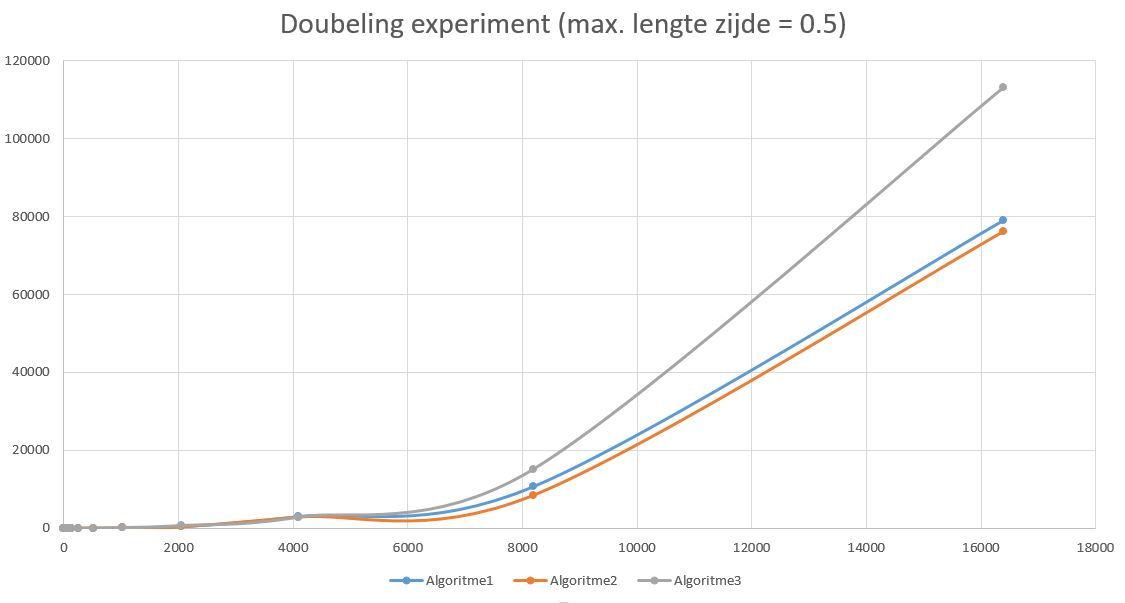
\includegraphics[width=0.75\textwidth]{zijde05.JPG}
				\caption{\label{fig:convR}Grafiek voor het doubeling experiment met zijdes die variëren tussen 0 en 0.5}
				\end{figure}
			
			
	\section{Bespreking resultaten}
	
\end{document}